\documentclass[11pt, a4paper]{article}
\usepackage[english]{babel}
\usepackage{natbib}
\usepackage{longtable}
\usepackage{caption}
\usepackage{subcaption}


\setlength{\parindent}{0em}
\setlength{\parskip}{1em}
\renewcommand{\baselinestretch}{1.5}
\usepackage[a4paper,left=2cm,right=2cm,top=2.5cm,bottom=2.5cm]{geometry}

\usepackage{fullpage}
    \usepackage{mathtools}
\usepackage{graphics}
\usepackage{amsmath}
\usepackage{float}
\usepackage{booktabs}
\usepackage{listings}
\usepackage{amsthm}
\usepackage{tikz}
\usetikzlibrary{calc}
\usepackage{xfrac}
\usepackage{mdframed}
\usepackage{scrextend}
\usepackage{natbib}
 
\begin{document}

\title{Iacoviello (2005) Basic Replication}
\author{Jack Minchin}
\date{11/03/2021}
\maketitle


\section{Introduction}

This is a simple replication of \cite{10.1257/0002828054201477}. It explores the impact of changing loan-to-value (LTV) rates in response to house price, inflation, monetary policy and technology shocks. 

	\section{Model}
	
	The model includes two types of households, savers and borrowers. Borrowers are relatively more impatient than saves to $\tilde\beta < \beta$. There are a continuum of final good firms who bundle intermediate goods, and intermediate goods firms who use labour to create an intermediate good that trades in a monopolistically competitive market. Intermediate firms are subject to a  time-dependent pricing model, following \cite{Calvo1983}.
	
	\subsection{Households}
	
	\subsubsection{Savers - Unconstrained Households}
	
	The unconstrained households are savers. Their maximisation problem is:
	\begin{equation}
\max E_{0} \sum_{t=0}^{\infty} \beta^{t}\left(\ln C_{t}^{u}+j \ln H_{t}^{u}-\frac{\left(L_{t}^{u}\right)^{\eta}}{\eta}\right),
\end{equation}
where $1 / (\eta -1)$ is the labour supply elasticity. $\eta > 0$ and $j >0$. $H_u$ is the amount of 'housing services' consumers by the savers, and $j$ denotes a weighting term for household. Everything else is standard.

The budget constraint is:
\begin{equation}
C_{t}^{u}+q_{t}\left(H_{t}^{u}-H_{t-1}^{u}\right)+b_{t}^{u} \leq w_{t}^{u} L_{t}^{u}+\frac{R_{t-1} b_{t-1}^{u}}{\pi_{t}}+F_{t}
\end{equation}

The FOC for savers are:
\begin{equation}
  \frac{j}{H^{u}_t} = \frac{1}{C^{u}_{t}} q_t - \beta \frac{1}{C^{u}_{t+1}} q_{t+1}
\end{equation}
\begin{equation}
  w_t^u = {L_t^{u}}^{\eta -1} C^u_t
\end{equation}
\begin{equation}
\frac{1}{C_{t}^{u}}=\beta E_{t}\left(\frac{R_{t}}{\pi_{t+1} C_{t+1}^{u}}\right)
\end{equation}


\subsubsection{Collateral Constrained Households}

We suppose the constrained households are relatively more impatient than the unconstrained households so that $\tilde\beta < \beta$. The problem of these households is:
\begin{equation}
\max E_{0} \sum_{t=0}^{\infty} \widetilde{\beta}^{t}\left(\ln C_{t}^{c}+j \ln H_{t}^{c}-\frac{\left(L_{t}^{c}\right)^{\eta}}{\eta}\right)
\end{equation}
subject to the budget constraint:
\begin{equation}
C_{t}^{c}+q_{t}\left(H_{t}^{c}-H_{t-1}^{c}\right)+\frac{R_{t-1}^{c} b_{t-1}^{c}}{\pi_{t}} \leq w_{t}^{c} L_{t}^{c}+b_{t}^{c}
\end{equation}
and the collateral constraint:
\begin{equation}
b_{t}^{c} \leq \frac{m}{R_{t}} E_{t} \pi_{t+1} q_{t+1} H_{t}^{c}
\end{equation}

This household has the FOCs:
\begin{equation}
\frac{1}{C_{t}^{c}}=\widetilde{\beta} E_{t}\left(\frac{R_{t}}{\pi_{t+1} C_{t+1}^{c}}\right)+\lambda_{t} R_{t}
\end{equation}
\begin{equation}
w_{t}^{c}=\left(L_{t}^{c}\right)^{\eta-1} C_{t}^{c}
\end{equation}
\begin{equation}
\frac{j}{H_{t}^{c}}=\frac{1}{C_{t}^{c}} q_{t}-\widetilde{\beta} E_{t} \frac{1}{C_{t+1}^{c}} q_{t+1}-\lambda_{t} m E_{t} q_{t+1} \pi_{t+1}
\end{equation}

Because the collateral constraint is binding, consumption for constrained households can be written as:
\begin{equation}
C_{t}^{c}=w_{t}^{c} L_{t}^{c}+b_{t}^{c}+q_{t}\left(H_{t-1}^{c}-H_{t}^{c}\right)-\frac{R_{t-1} b_{t-1}^{c}}{\pi_{t}}
\end{equation}
and the FOC becomes:
\begin{equation}
\frac{j}{H_{t}^{c}}=\frac{1}{C_{t}^{c}}\left(q_{t}-\frac{m E_{t} q_{t+1} \pi_{t+1}}{R_{t}^{c}}\right)-\widetilde{\beta} E_{t} \frac{1}{C_{t+1}^{c}}(1-m) q_{t+1}
\end{equation}

\subsection{Firms}

%%% ******************************************************************************************************** %%%
%%% ******************************************  Final Goods Firms ****************************************** %%%
%%% ******************************************************************************************************** %%%

\subsubsection{Final Goods Firms}

There are a continuum of final goods firms bundle together intermediate goods to produce a final good. 
\begin{equation}
Y_{t}=\left[\int_{0}^{1} Y_{t}(z)^{\frac{\varepsilon-1}{\varepsilon}} d z\right]^{\frac{\varepsilon}{\varepsilon-1}}
\end{equation}
subject to the market clearing condition.
\begin{equation}
Y_{t}=C_{t}=C_{t}^{u}+C_{t}^{c}
\end{equation}


The demand for the intermediate goods can be found to be:
\begin{equation}
  Y_{it}^d =\left[\frac{P_t}{P_{it}}\right]^\frac{1}{1-q} Y_t
\end{equation}



%%% ******************************************************************************************************** %%%
%%% ******************************************  Intermediate Firms ***************************************** %%%
%%% ******************************************************************************************************** %%%

\subsubsection{Intermediate Goods Firms}

Intermediate goods firms combine labour to create an intermediate good that is traded on a monopolistically competitive market. Following Cavlo (1983), only a proportion $\omega$ of firms can change their price each period.

The intermediate firms face a simple production function:
\begin{equation}
  Y_{it} = A_t {L_t^u}^ \eta + {L^c_t}^{1-\eta}
\end{equation}
where $A_t$ follows an AR(1) procces. The profit function for the intermediate goods firms is:
\begin{equation}
  \min_{L^u, L^c} \Pi_{it} = w_c L_u + w_c L_c
\end{equation}
subject to the production function. 

From this, we can find the conditions for wages:

\begin{equation}
  w_{ut} = \eta (-A_t)\frac{1}{X}L^{\eta-1}
\end{equation}
and:
\begin{equation}
 w_{ct} = (\eta -1) (-A_t)\frac{1}{X}L^{-\eta}
\end{equation}






%%% ******************************************************************************************************** %%%
%%% ******************************************  Monetary Policy ******************************************** %%%
%%% ******************************************************************************************************** %%%


\subsection{Monetary Policy}

Closing the model with the Taylor rule and the New Keynesian Phillips Curve.
\begin{equation}
\pi_{t}=\beta E_{t} \pi_{t+1}+\kappa \hat{\nu}_{t}
\end{equation}
$\kappa$ is $\frac{(1-\omega)(1-\beta \omega)}{\omega}$.

\begin{equation}
	r_{t}=\phi_{r} r_{t-1}+\left(1-\phi_{r}\right)\left(\left(1+\phi_{\pi}\right) \pi_{t}+\phi_{z} z_{t}\right)+e_{t}
\end{equation}




%%% ******************************************************************************************************** %%%
%%% ******************************************      Results     ******************************************** %%%
%%% ******************************************************************************************************** %%%

\section{Results}

\subsection{House Price Shocks}
\begin{figure}[H]\centering
  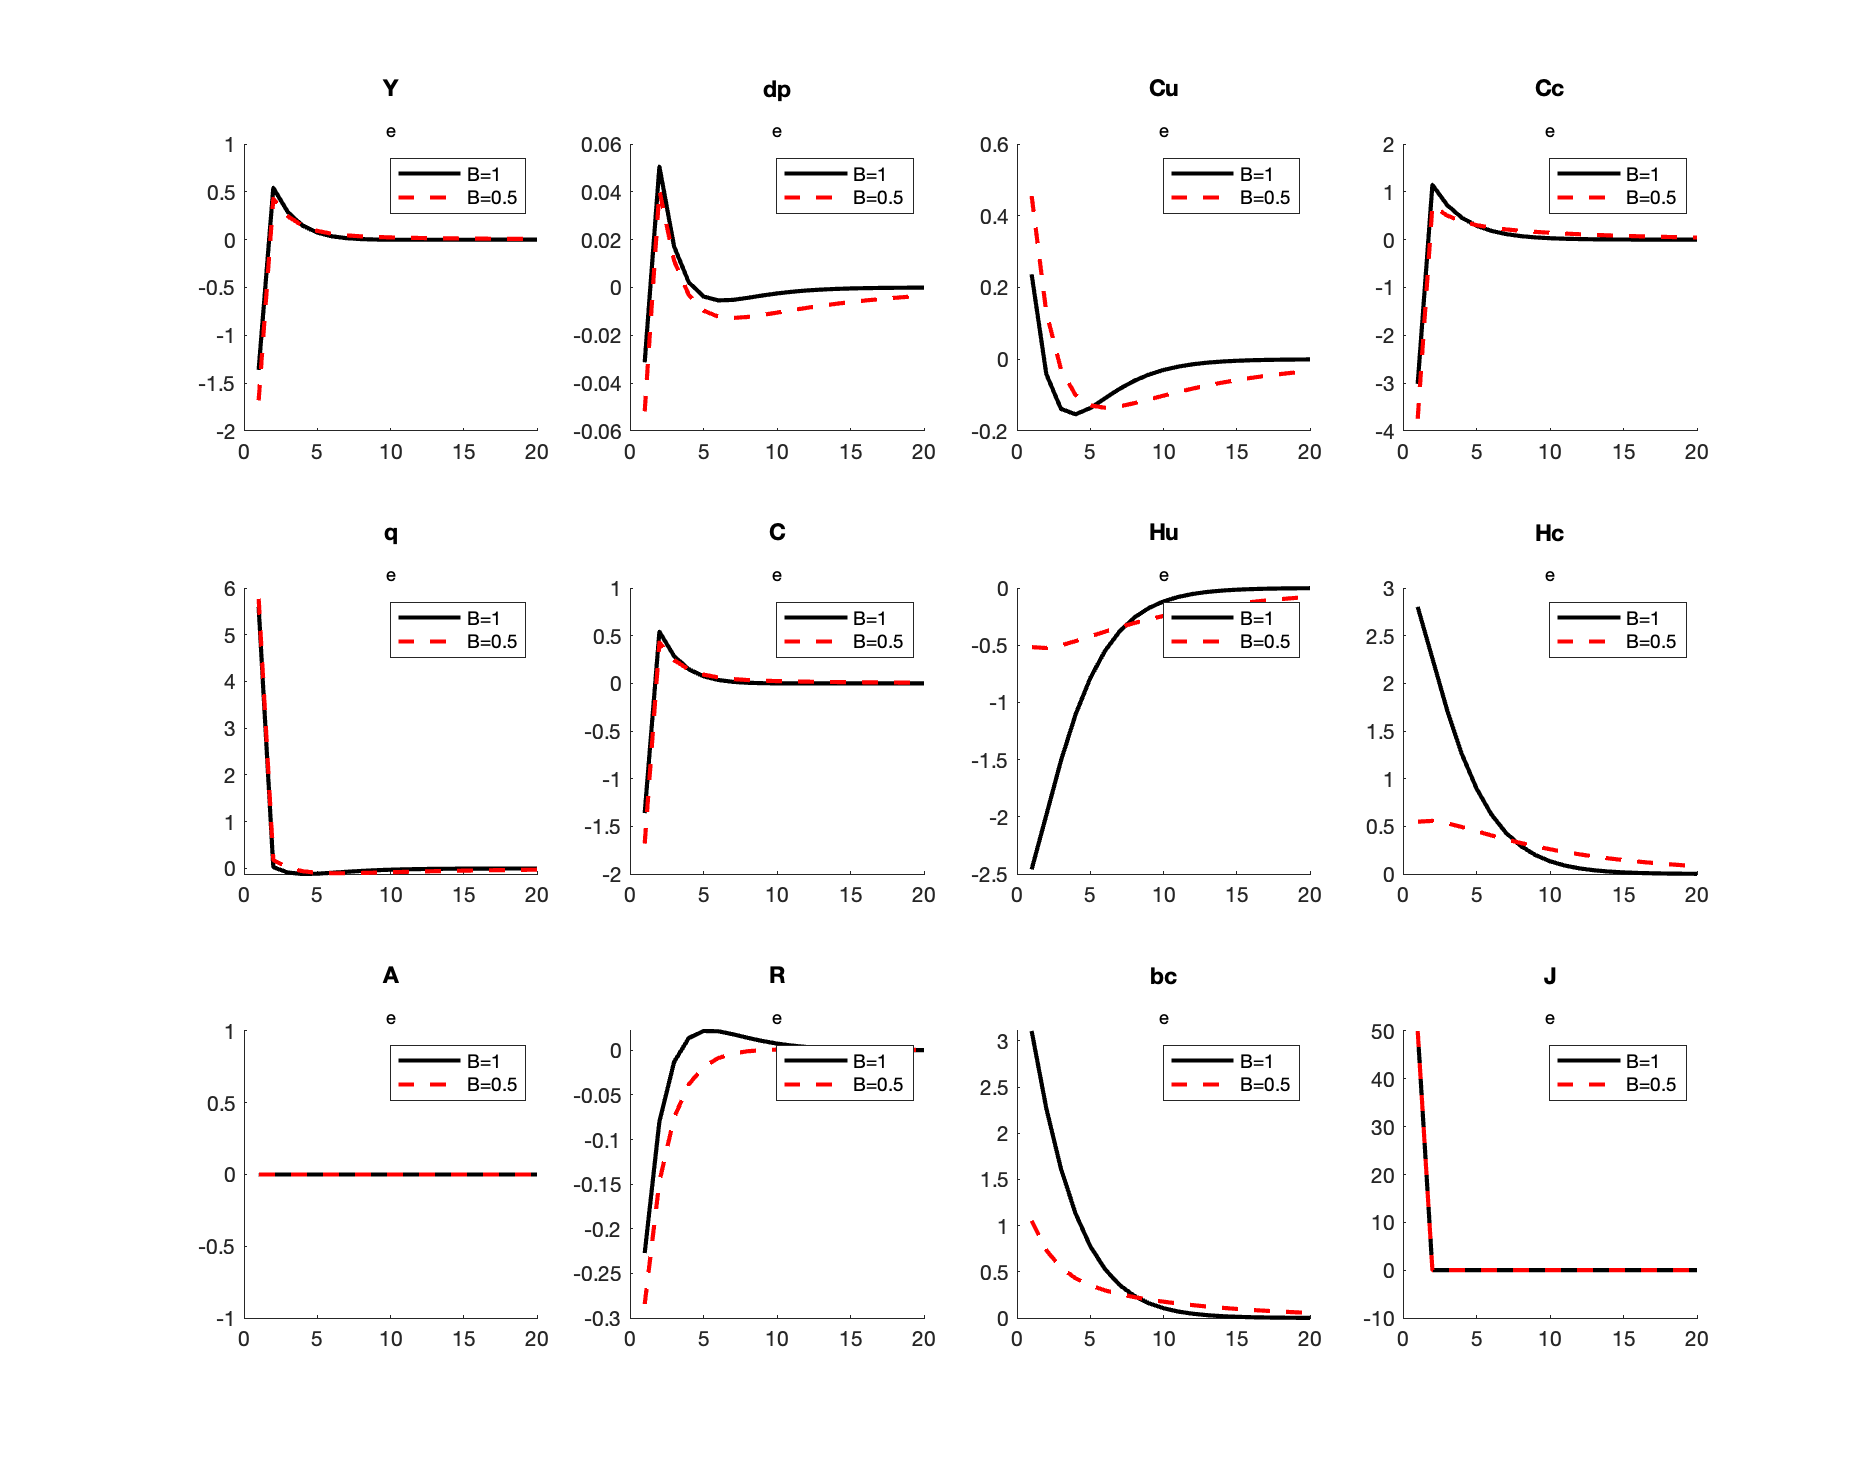
\includegraphics[scale=0.5]{../figs/_e}
  \caption{}
\end{figure}

\subsubsection{Monetary Policy Shock}
\begin{figure}[H]\centering
   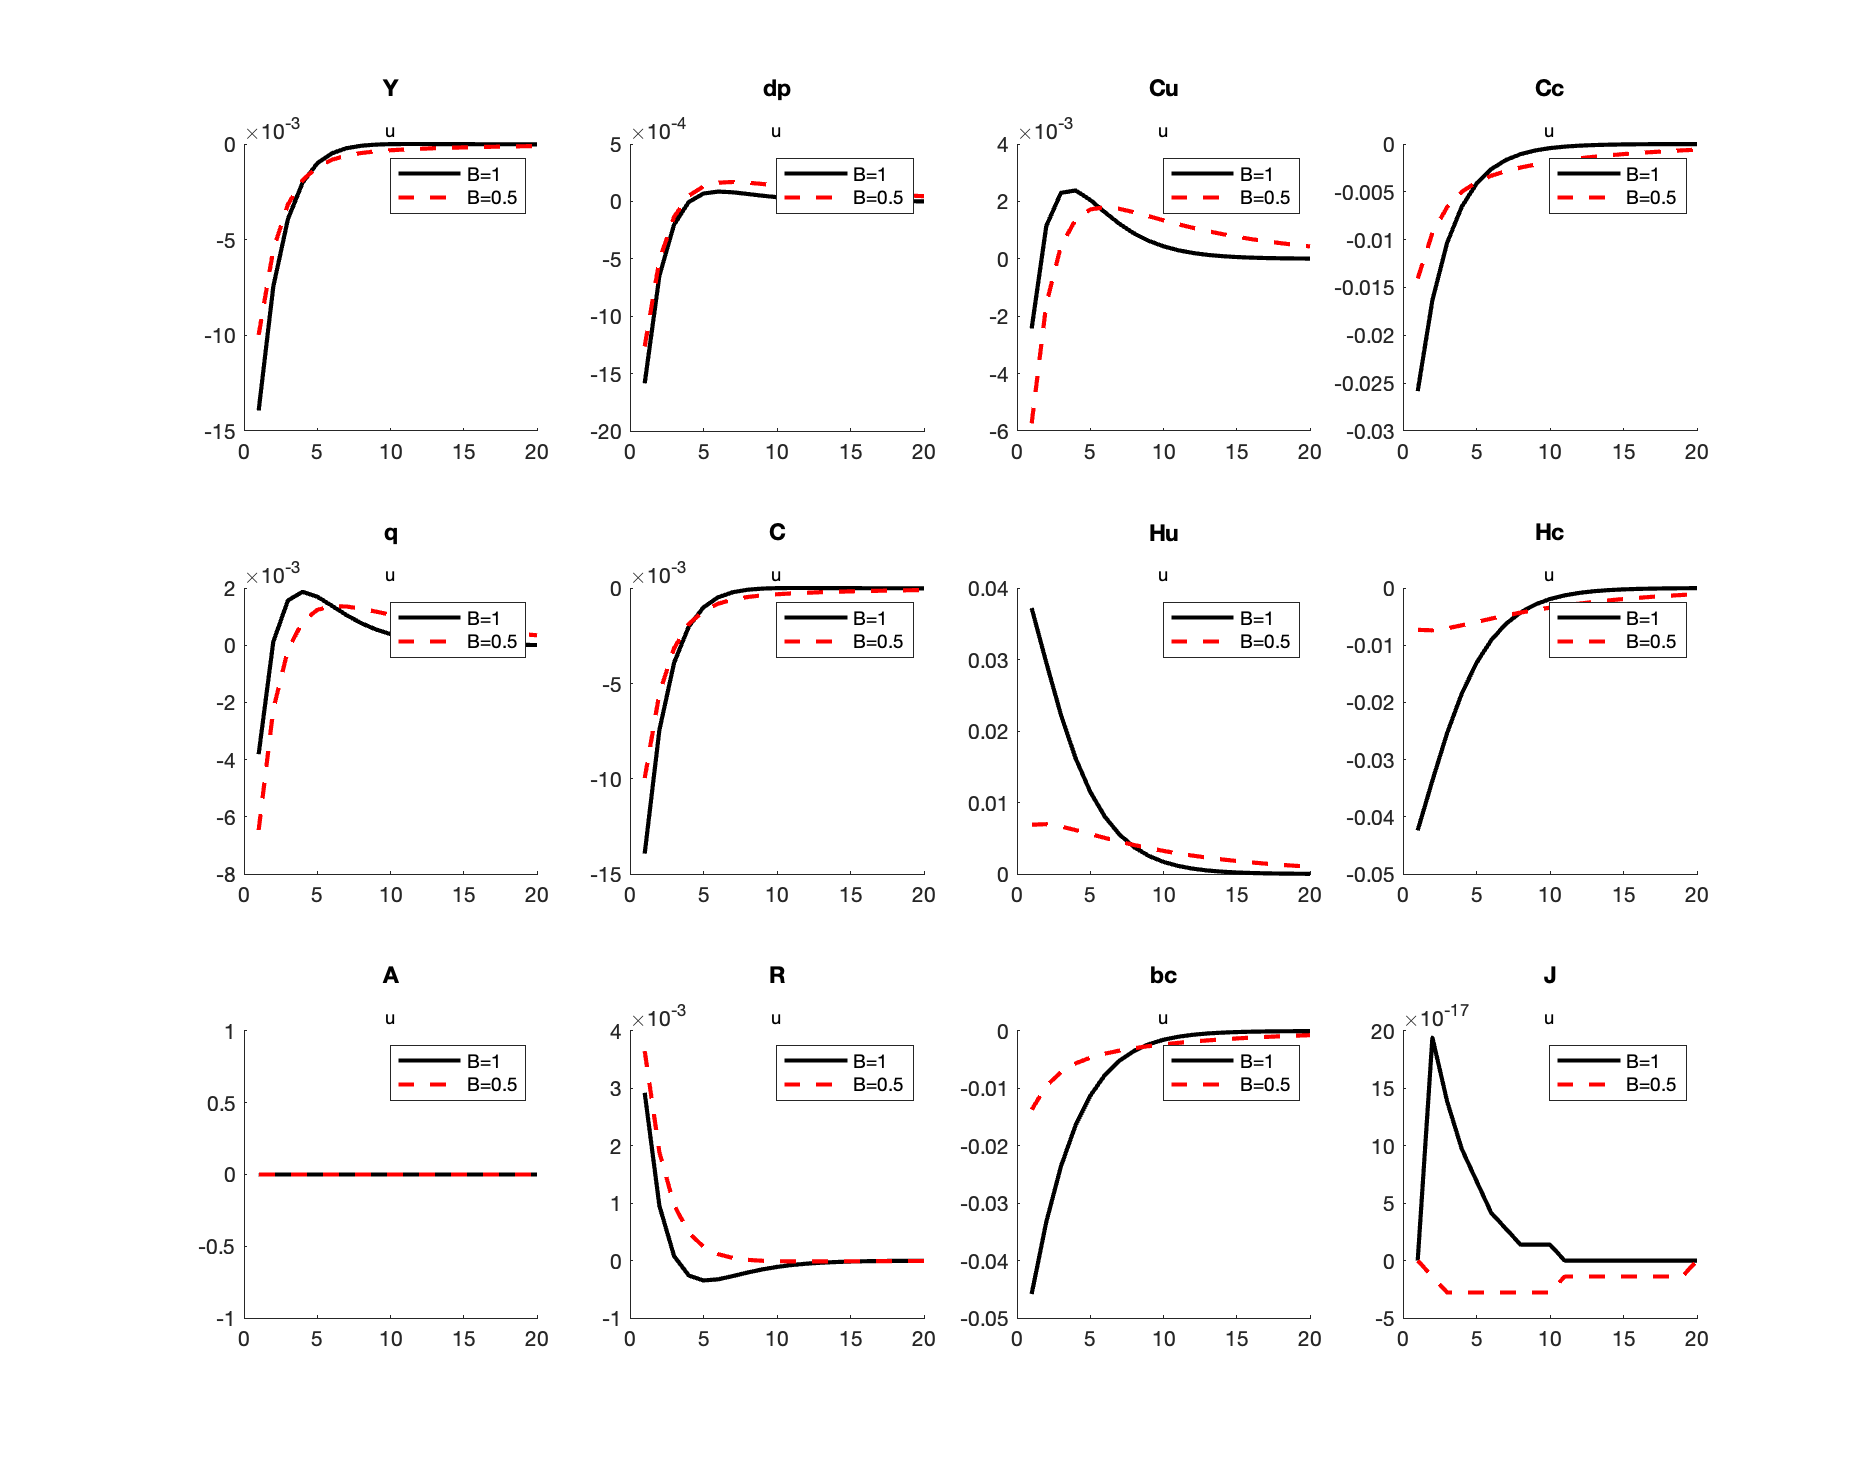
\includegraphics[scale=0.5]{../figs/_u}
  \caption{}
\end{figure}

\subsubsection{Technology Shock}
\begin{figure}[H]\centering
  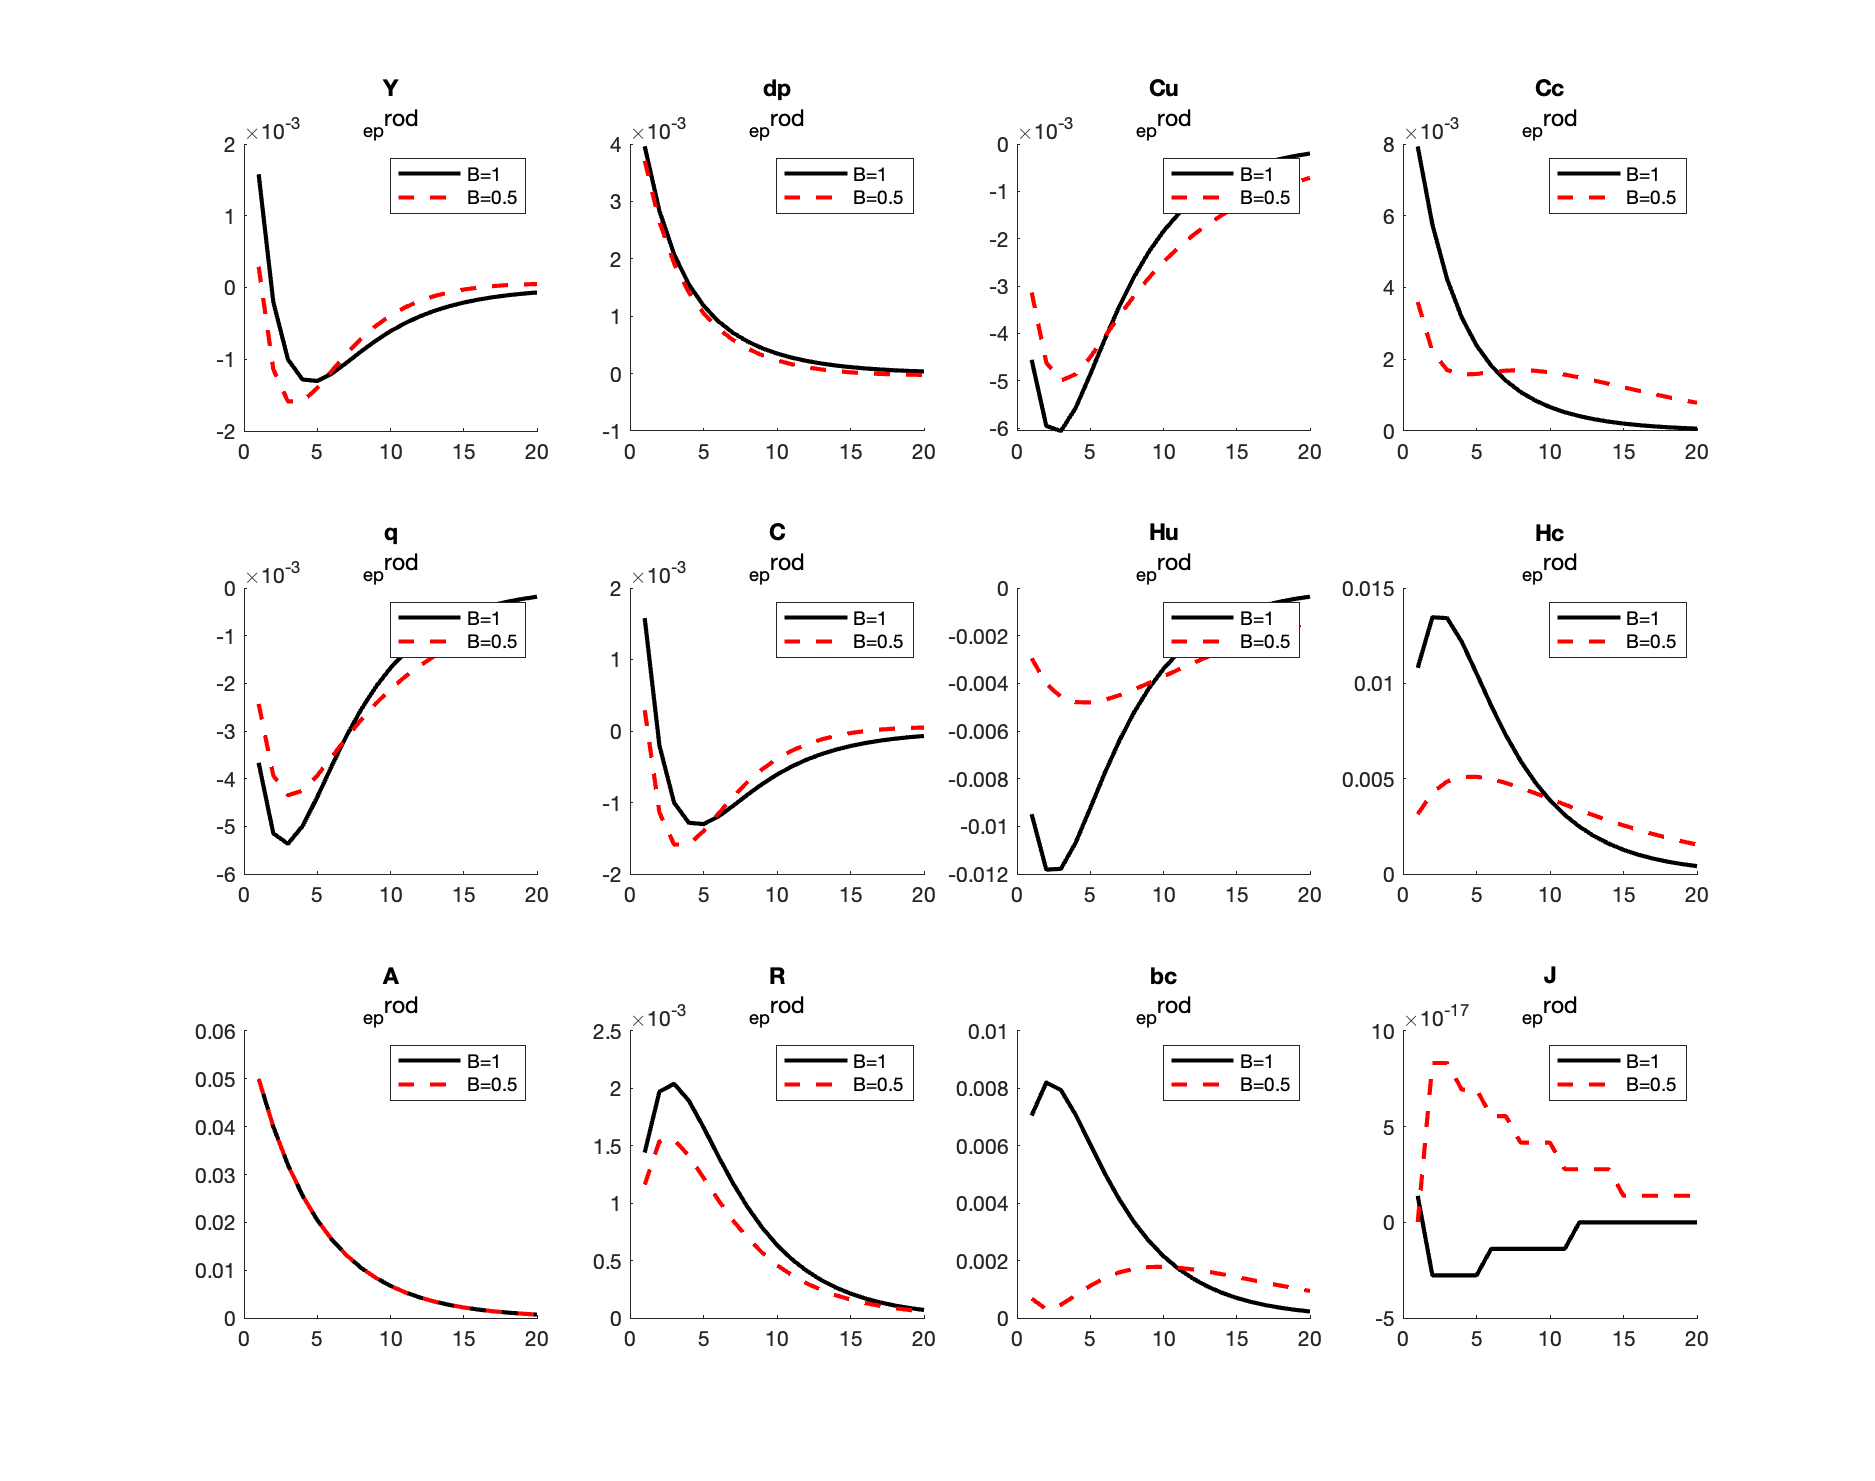
\includegraphics[scale=0.5]{../figs/_e_prod}
  \caption{}
\end{figure}

\subsubsection{Cost-Push Inflationary Shock}
\begin{figure}[H]\centering
  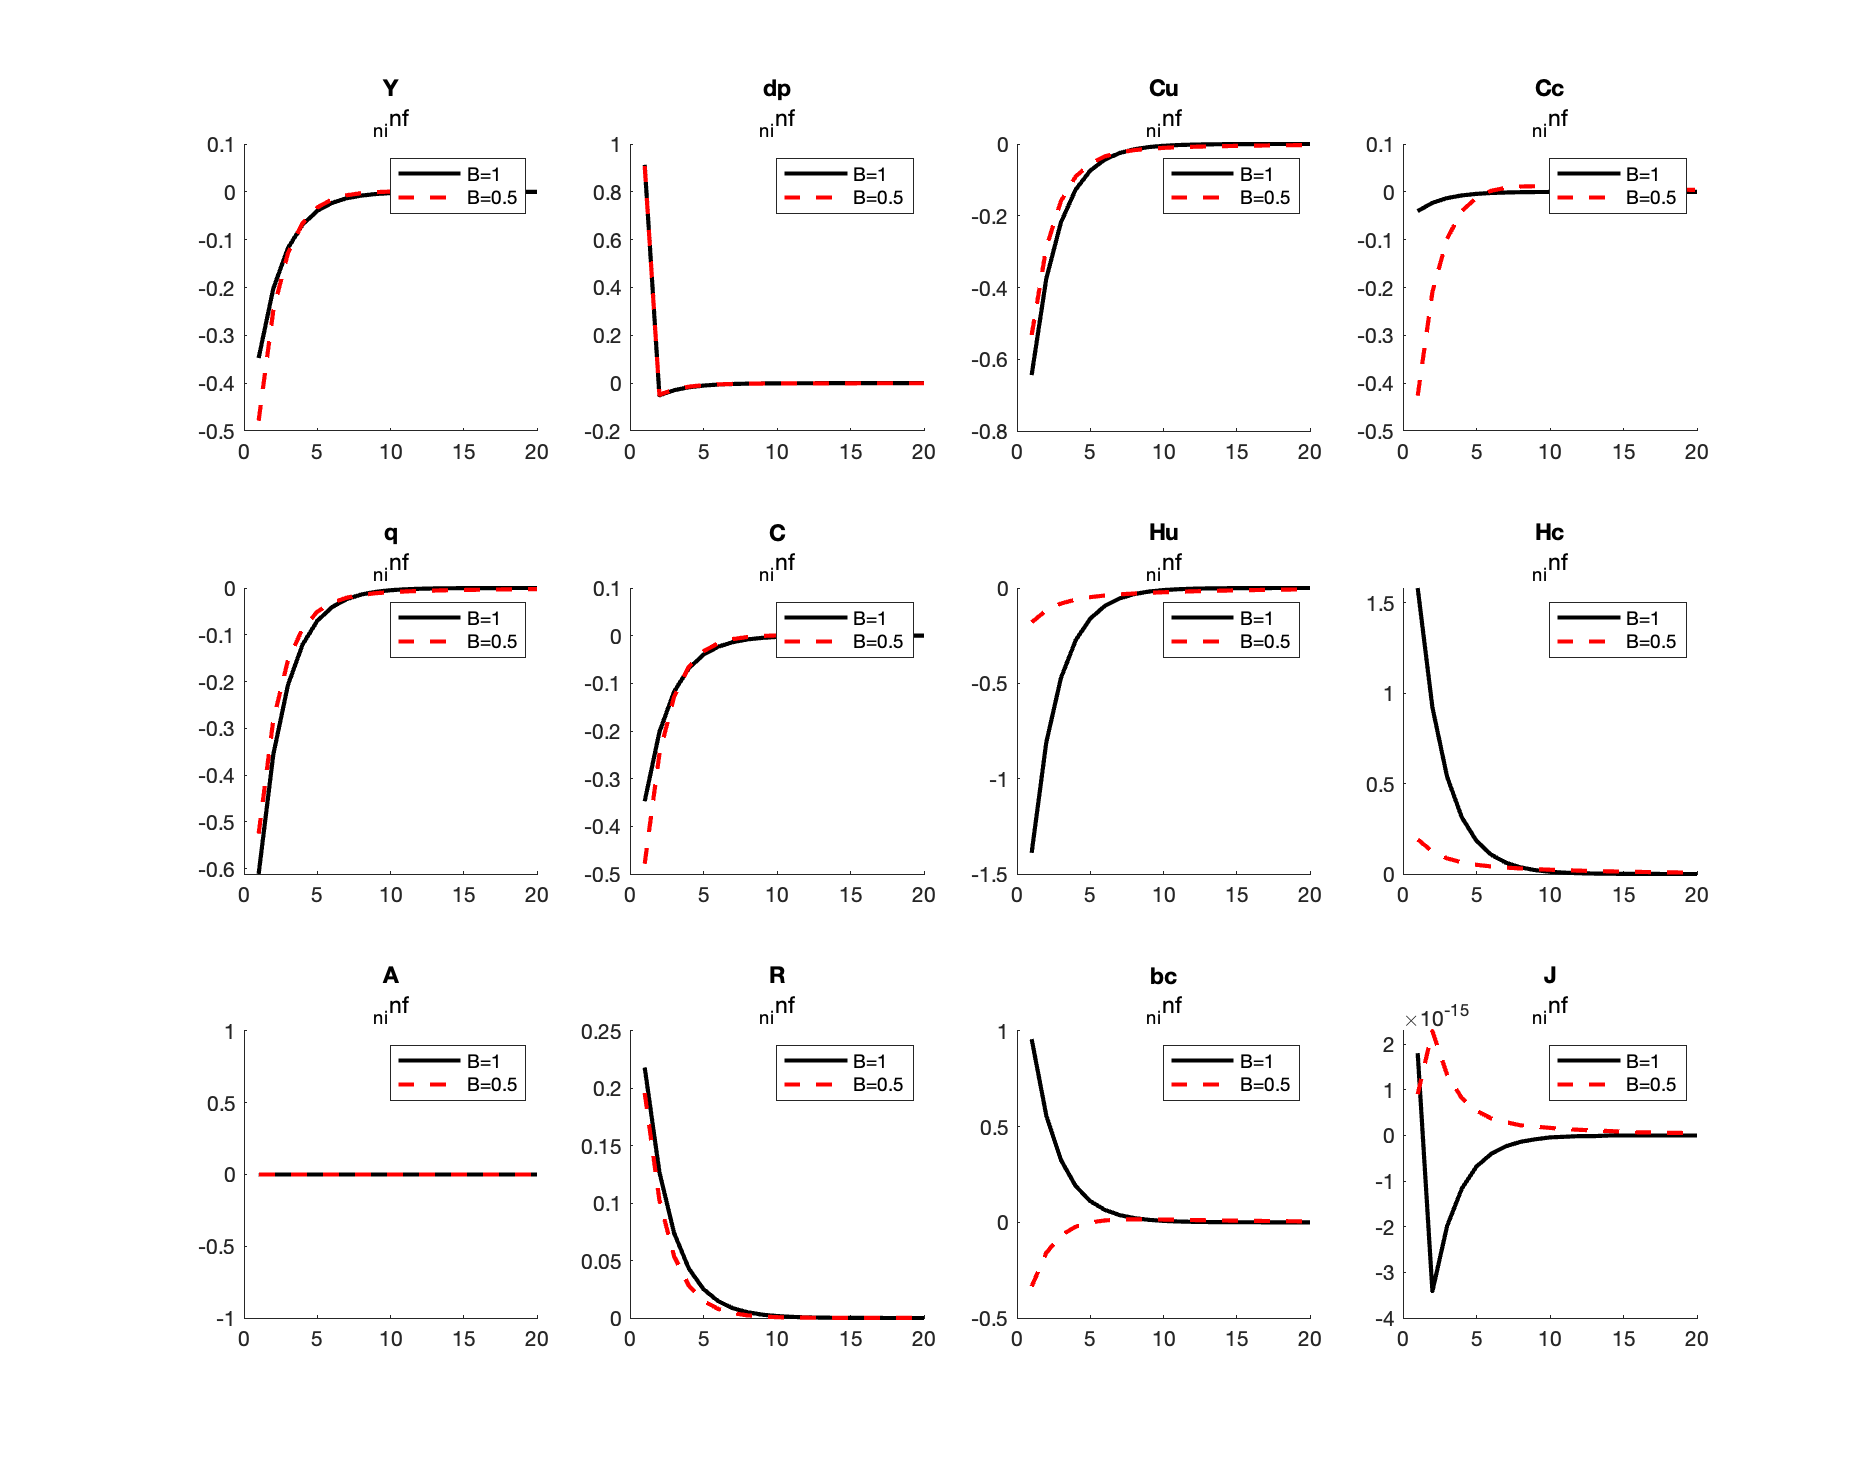
\includegraphics[scale=0.5]{../figs/_n_inf}
  \caption{}
\end{figure}

\bibliographystyle{humannat}
\bibliography{../../../../Documents/library.bib}


%%% ******************************************************************************************************** %%%
%%% ******************************************  APPENDIX        ******************************************** %%%
%%% ******************************************************************************************************** %%%

\section*{Appendix}
\subsection*{Households}

The Lagrangian for the unconstrained household problem is:
\begin{equation}
\begin{aligned}
  \mathcal{L} = \ln C^u_t + j  \ln H^u - \frac{\left(L_{t}^{u}\right)^{\eta}}{\eta} + \dots \\
  - \lambda_t \bigg(C_{t}^{u}+q_{t}\left(H_{t}^{u}-H_{t-1}^{u}\right)+b_{t}^{u} - w_{t}^{u} L_{t}^{u}+\frac{R_{t-1} b_{t-1}^{u}}{\pi_{t}}+F_{t}\bigg)  \\- \beta \lambda_{t+1} \bigg(C_{t+1}^{u}+q_{t+1}\left(H_{t+1}^{u}-H_{t}^{u}\right)+b_{t+1}^{u} - w_{t+1}^{u} L_{t+1}^{u}+\frac{R_{t} b_{t}^{u}}{\pi_{t+1}}+F_{t}+1\bigg)
  \end{aligned}
\end{equation}

To get the FOCs, we maximise w.r.t consumption, labour, housing and the Lagrange multiplier to get: 

\begin{equation}
  \frac{j}{H^{u}_t} = \frac{1}{C^{u}_{t}} q_t - \beta \frac{1}{C^{u}_{t+1}} q_{t+1}
\end{equation}
\begin{equation}
  w_t^u = {L_t^{u}}^{\eta -1} C^u_t
\end{equation}
\begin{equation}
\frac{1}{C_{t}^{u}}=\beta E_{t}\left(\frac{R_{t}}{\pi_{t+1} C_{t+1}^{u}}\right)
\end{equation}

\subsection*{Intermediate Firms}

\begin{equation}
  \min_{L^u, L^c} \Pi_{it} = w_u L_u+ w_c L_c
\end{equation}
subject to:
\begin{equation}
  Y_{it} = A_t {L_t^u}^ \gamma {L^c_t}^{1-\gamma}
\end{equation}
\begin{equation}
\begin{aligned}
  \mathcal{L} = w_uL_u + w_cL_c  - Z_t\left(Y_{it} - A_t {L_{ut}}^ \gamma {L_{ct}}^{1-\gamma}\right)
  \end{aligned}
\end{equation}

\begin{equation}
  \frac{\partial \mathcal{L}}{L_u} = 0  \rightarrow w_{ut} = \gamma A_t \frac{1}{X} L_{ct}^{(1-\gamma)}L_{ut}^{\gamma-1}
\end{equation}

\begin{equation}
  \frac{\partial \mathcal{L}}{L_c} = 0  \rightarrow w_{ct} = (\gamma -1) (-A_t)\frac{1}{X}L_{ct}^{-\gamma}L_{ut}^\gamma
\end{equation}





\end{document}
